% status: 100
% chapter: Amazon

\title{Amazon AWS EC2}


\author{Sushant Athaley}
\affiliation{%
  \institution{Indiana University}
}
\email{sathaley@iu.edu}

% The default list of authors is too long for headers}
\renewcommand{\shortauthors}{G. v. Laszewski}


\begin{abstract}
AWS EC2 is a cloud infrastructure offering from Amazon which provides compute resource virtualization. We explore AWS EC2 technology to understand how we can use compute resource in a cloud environment. 

\end{abstract}

\keywords{hid-sp18-402, i516, Amazon, AWS, EC2, Cloud, VM}

\maketitle

\section{Introduction}
The emergence of cloud computing is changing the paradigm the way we are working with IT resources. It is helping to virtualize various IT resources and eliminating the need for in-premise infrastructure. EC2 is one such service which provides computation capability in the cloud. We evaluate EC2 as technology to understand various feature provided by the service and how it is getting used to solve practical problems.

We get started with the section \emph{Cloud} which explains the concept of Cloud and various cloud offerings. Section \emph{EC2} provides an introduction to the EC2 technology. Then we explore technology in detail through subsections \emph{E-Elastic} which captures elasticity in EC2, \emph{Instances and AMIs} captures various software and hardware options, \emph{Integrated} captures integration information, \emph{Security} explains security features provided, \emph{Storage} explores various storage options and \emph{Pricing} captures pricing information to use EC2.
Section \emph{Working with EC2} explores various ways to work with EC2. Section \emph{Real Life Use Cases} talks about real life EC2 usage examples. Section \emph{Conclusion} concludes the study. 

\section{Cloud}
In order to understand EC2, it's imminent that we understand the concept of Cloud as EC2 is nothing but a cloud offering and it is backed up by various feature and benefits provided by the Cloud technology.  Term \emph{Cloud} comes from the way internet is shown as a cloud in various software diagram, so Cloud's one of the easiest interpretation is something which can be done over the internet instead of using our own CPU or storage \cite{www-infoworld}. It is the new concept where instead of using the traditional way of setting up IT infrastructure to get the IT work done and then maintain it, infrastructure commercially developed, is used remotely over the internet. It virtualizes and centralizes the whole IT infrastructure required by the enterprise. Cloud is often backed up by massive infrastructure which provides the ability to quickly upscale and downscale the required resources like compute, storage and network and can use proven ready to use pre-build services. Customer perspective, cloud enables them to get new capabilities on demand without bothering about analysis and investment need to be made on procuring new software or hardware. It cuts down on the time involved to create the infrastructure as this resources are already pre-build and readily available for use through the cloud and can be set up within minutes for the usage. Addition of resources or scaling down on the resources automatically based on a demand is the biggest advantage. Instead of paying for entire infrastructure at once, cloud provides an option to pay per use which might be the cheaper alternative.

There are various cloud services available like Software as a Service (SaaS), Infrastructure as a Service (IaaS), Platform as a Service (PaaS) and Function as a Service (FaaS) \cite{www-infoworld}. The topic of this study, EC2 is IaaS offering and provides compute capability in the Amazon AWS environment.


\section{EC2}
EC2 is the commercial web service offering from Amazon. Amazon describes Elastic Compute Cloud which is referred as EC2 is a web service which provides compute capacity in the cloud along with security and re-size features \cite{www-aws-ec2}. In layman term, we can think of it as a virtual computer in the cloud which can be used for any task which can be performed using a physical computer. It can be used as server, development instance, personal computer, deployment environment, test environment, virtual machine or many more depending on the need. The EC2 instance can have an operating system from the variety of the range available like Windows, Amazon Linux, CentOS, and Debain along with the option of uploading your own operating system \cite{www-aws-ec2-details}. EC2 instance can be loaded with a custom application environment as well as can be used to work with various AWS or other services. As this is a cloud offering it comes with various benefits offered by the cloud technology as well as the massive infrastructure provided by Amazon.

\subsection{E-Elastic}
E in EC2 stands for Elastic which enables to increase and decrease capacity on demand but also maintains the desired capacity. It can be used to commission hundred to thousand instances simultaneously based on the requirement \cite{www-aws-ec2}. This is one of the great features as it helps to control computing power needed based on the demand and provides optimized performance. 
Amazon EC2 Auto Scaling \cite{www-aws-ec2autoscaling} feature enables to configure various rules which are used to maintain or scale the instances. 
\subsubsection{Fleet Management}
EC2 Auto Scaling offers \emph{Fleet Management} which periodically monitors the health of running instance and replaces faulty instance automatically by terminating that instance and replacing it with the new instance. The number of instances can be configured in the fleet and auto-scaling will ensure that those number of instances are up and running all the time without any downtime or impact to the users.
\subsubsection{Dynamic Scaling}
Dynamic Scaling enables to increase or decrease the capacity based on a parameter like CPU utilization where new instance will be added or removed after certain CPU utilization is reached. This mechanism helps to balance the load and provide the optimized performance to the users as well as save cost by optimizing the resources.

Figure \ref{f:ec2-auto-scaling} shows EC2 Auto Scaling
\begin{figure}[!ht]
  \centering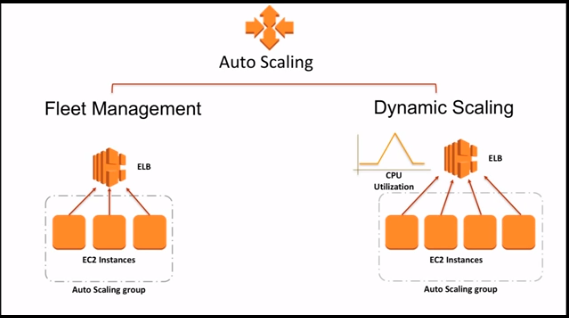
\includegraphics[width=\columnwidth]{images/ec2AutoScaling.PNG}
  \caption{EC2 Auto Scaling \cite{www-aws-ec2autoscaling}}\label{f:ec2-auto-scaling}
\end{figure}

\subsection{Instances and AMIs}
EC2 provides flexibility to use the variety of instances which is based on CPU, memory, storage, and the networking capability. Each instance type provides the various combination of those parameters to choose appropriate computing capability required as per the use case. This helps in optimizing resources and cost based on the workload. These instances are divided into various categories as General Purpose, Compute Optimized, Memory Optimized, Storage Optimized and Accelerated Computing. To get an idea of instance type provided by EC2, for example in general category the smallest instance type \emph{t2.nano} would look like as 1 vCPU, 0.5GB memory, low networking performance with Intel Xeon processor 3.3GHz whereas the higher end instance type combination \emph{m4.16xlarge} is 64vCPU, 256GB memory, 25GB networking speed with Intel Xeon E5-2686v4 processor 2.3GHz \cite{www-aws-ec2instance}. There are lot many other options based on the different parameters which can be readily picked up and deployed as EC2 instance without waiting for hardware procurement.

Amazon Machine Image (AMI) \cite{www-aws-ec2instance} is a pre-configured image of the required operating system, software, servers, databases, and applications. AMI is used to launch an instance which in turn uses selected AMI to run on the instance. There are predefined AMIs which can be readily used but also custom AMI can be created based on the requirement.

Figure \ref{f:ec2-ami-instance} shows EC2 AMI and Instance relationship
\begin{figure}[!ht]
  \centering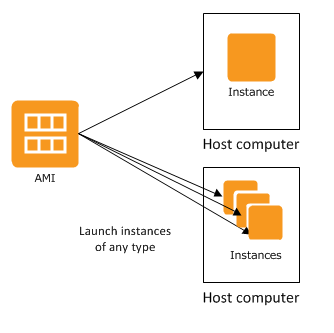
\includegraphics[width=\columnwidth]{images/ec2AMI.PNG}
  \caption{EC2 Instance and AMI \cite{www-aws-ec2instance}}\label{f:ec2-ami-instance}
\end{figure}

\subsection{Integrated}
EC2 is backed by various services offered by AWS and can be integrated with those services. AWS S3, AWS RDC, AWS VPC are some of the services which can be used in conjunction with EC2 to develop different applications \cite{www-aws-ec2}.
Figure \ref{f:ec2-integration} shows sample EC2 integration with S3, RDS and EBS 
\begin{figure}[!ht]
  \centering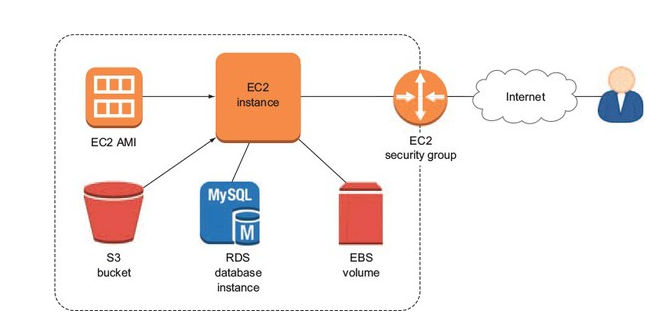
\includegraphics[width=\columnwidth]{images/ec2Integration.PNG}
  \caption{EC2 Integration \cite{www-medium-aws}}\label{f:ec2-integration}
\end{figure}

\subsection{Security}
Security in EC2 is provided on multiple levels, by the operating system on the instance, guest OS, firewall and signed API calls. Host operating system itself has security and access mechanism built in which can restrict unauthorized access. Guest OS itself is a less privileged access which doesn't allow critical operations. EC2 provides firewall solution which is used to restrict traffic on certain ports as well as for certain protocols and IP addresses. Inbound traffic requires explicitly port opening and specific group policy can be applied to access those ports. Remote access through API calls can only be made if secret access key is created and established using EC2 \cite{www-aws-ec2Security}.

\subsection{Storage}
Data storage and processing are essential capabilities for many of the compute operations. EC2 provides various options for the data storage and those options have their own characteristics in terms of performance and durability \cite{www-aws-ec2Storage}. Figure \ref{f:ec2-storage} shows relationship between various storage type provided by EC2
\begin{figure}[!ht]
  \centering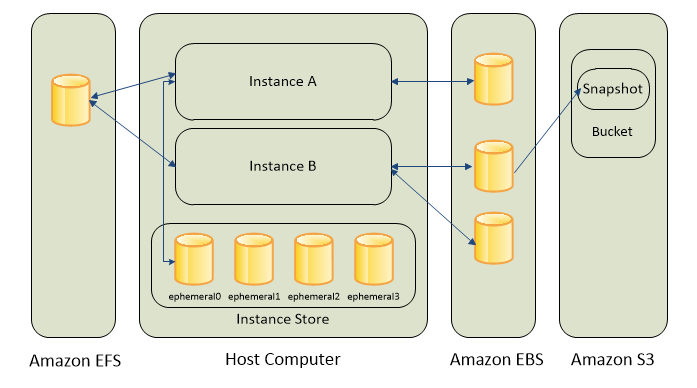
\includegraphics[width=\columnwidth]{images/ec2Storage.PNG}
  \caption{EC2 Storage Types \cite{www-aws-ec2Storage}}\label{f:ec2-storage}
\end{figure}

\subsubsection{Amazon EC2 Instance Store} 
Instance store \cite{www-aws-ec2Storage} is the temporary storage attached as a physical disk to the host computer. This can be used for the temporary storage like buffer, cache, scratch data as it is lost in case of instance stopped, terminated or disk drive is failed.
\subsubsection{Amazon Elastic Block Store (EBS)} 
EBS provides durable, block-level storage to the EC2 instance. This storage is independent of instance life cycle and can be used as primary storage type for the EC2. This is persistent storage and can be attached to multiple instances. EBS can be used as database storage. It also provides encryption capabilities \cite{www-aws-ec2Storage}.
\subsubsection{Amazon Elastic File System (EFS)} 
EFS provides file system storage to the EC2 instance \cite{www-aws-ec2Storage}. This is a persistent storage which can be used or shared between multiple instances.
\subsubsection{Amazon Simple Storage Service (S3)} 
S3 is persistent and instance independent data store which is suitable for data movement and storage in large volume. This storage can be accessed through EC2 as well as from outside over the web \cite{www-aws-ec2Storage}. 

\subsection{Pricing}
EC2 is a commercial offering from Amazon and it offers various pay models which can be used as per the need. It also offers free option to try if the micro instance is used.
\subsubsection{On-Demand} 
This option allows to pay on per hour or per second basis based on the instance usage \cite{www-aws-ec2Pricing}.
\subsubsection{Spot Instances} 
Spot instances are the spare instances and offered at steep discounts based on the biding. Spot instance can be interrupted at any point if the EC2 instance needs its capacity back \cite{www-aws-ec2Pricing}.
\subsubsection{Reserved Instances} 
Reserved instance offers discounted rates compared to on-demand rates based on the commitment provided by the customer. Reserved instance provides capacity reservation to launch instance as required which ensures the instance availbility \cite{www-aws-ec2Pricing}.
\subsubsection{Dedicated Hosts} 
A dedicated host provides the dedicated physical EC2 instance for the usage. This can be useful if any compliance or regulatory requirement needs to be met by the business \cite{www-aws-ec2Pricing}.

\section{Working with EC2}
There are 3 different ways which can be used to interact with EC2. To use EC2, first we need to create AWS account and then complete related setup like creation of IAM (Identity and Access Management) user to access, creation of key pair for secure access, creation of virtual private cloud (VPC) to lunch instance in user-defined virtual network and creation of security group which act as a firewall \cite{www-aws-ec2-setup}.

\subsection{Management Console}
Management Console \cite{www-aws-ec2-gettingStarted} is a web-based user interface to access various AWS resources. Log in to the management console and select EC2 from the list to get started. This interface provides the capability to configure the instance, launch the instance, connect to the instance and terminate the instance.

\subsection{Command Line Tool}
AWS CLI (Command Line Interface) \cite{www-aws-ec2-cli} is the command line interface provided by Amazon to interact with various AWS web services. This open source tool is built on top of the AWS SDK for Python. These commands can be used from Linux shells, windows command line and remotely through a remote terminal like PuTTY. To use AWS CLI, it needs to be installed using \emph{pip} on Linux, macOS, or Unix environment and on Windows using MSI installer. AWS CLI need to be configured by setting key and region before it can be used to work with the EC2 instance.
Figure \ref{c:cli-launch} shows sample CLI command to launch the instance, it is just for the information purpose only and need to update with correct parameter values to get executed in the specific environment
\begin{figure}[htb]
\begin{verbatim}
aws ec2 run-instances --image-id ami-6e1a0117
--security-group-ids sg-b018ced5 
--count 1 --instance-type t2.micro 
--key-name devenv-key 
--query 'Instances[0].InstanceId'
\end{verbatim}
\caption{Launch Instance \cite{www-aws-ec2-cli}}\label{c:cli-launch}
\end{figure}

\subsection{SDKs}
AWS services can be accessed through various platforms or programming languages which enables a developer to work with AWS in their preferred programming language. These platforms or language-specific libraries are called as SDK. Currently, SDKs are available for \emph{Android, Browser, iOS, Java, .Net, Node.js, PHP, Python, Ruby, Go,} and \emph{C++} \cite{www-aws-ec2-sdk}. 

\section{Real Life Use Cases}
Any technology can be understood better by understanding real-life examples of how it is being used practically to solve the problem or the use case. In this section, we explore some examples of EC2 usage from real life.

\subsubsection{Netflix}
Netflix is one of a good example of cloud platform usage as well as AWS usage. Netflix completed their migration to AWS cloud in 2016 which lasted over the period of 7 years \cite{www-media-netflix}. Netflix uses numerous services provided by AWS out of which EC2 is used as computing service which hosts Netflix's various customer facing as well as internal applications, Cassandra Database, Elasticsearch, and EVCache. It uses EC2 Linux cloud with thousands of virtual server instances along with the autoscale feature to support over 50M subscribers \cite{www-brendangregg}.

\subsubsection{Airbnb}
Airbnb is a community marketplace for finding the vacation rentals having more than 9 million users. They require massive storage along with the efficient rental booking application to support growing request load. Airbnb uses AWS EC2, elastic load balancing, EMR, S3, Cloudwatch, and Amazon RDS. It uses 200 EC2 instances for application hosting, memcache and search servers \cite{www-aws-ec2-airbnb}.

\subsubsection{Novartis}
Novartis is a pharmaceutical company involved in drug discovery and innovation. They wanted to run the complex algorithm to screen 10 million compounds against common cancer target which would require huge computing capability along with the storage. They used AWS EC2, S3, and EBS to built a program which ran on multiple instances simultaneously to complete the matching. They used 10,600 EC2 spot instances to run the algorithm \cite{www-aws-ec2-novartis}.

\subsubsection{Lamborghini}
Lamborghini is an automotive company which was facing issue with the outdated infrastructure and nonscalable environment they were using to host their website. They decided to migrate their website to AWS and used AWS ELB, EC2, RDS, S3, CloudFront, and Cloudwatch in their architecture \cite{www-aws-ec2-lamborghini}. It is not clear from the available documentation how they are using EC2 in their design but our guess is, EC2 is getting used as a web-server host for the web application.

\section{Conclusion}
EC2 is a commercial web service provided by Amazon. This is an Infrastructure as a Service (IaaS) cloud offering which provides compute capability. EC2 provides features like elastic auto-scaling, flexible hardware and software configurations, integrations with other AWS web services, access security using secure key and firewall configurations, data storage options and flexible price options. It also provides an interactive web interface to work with the EC2 instances at the same time SDKs in various programming languages to work with EC2 in a programmatic way. One of the biggest advantages of EC2 is the infrastructure provided by Amazon which helps to create thousands of instances in very less time which is helpful for solving big data or any other problems which require a lot of computing capability. The robust features and flexibility offered by EC2 makes it as preferred virtual compute resource.

\begin{acks}

  The author would like to thank Dr. Gregor von Laszewski for his
  support and suggestions to write this paper.

\end{acks}

\bibliographystyle{ACM-Reference-Format}
\bibliography{report} 
